\chapter{Implementation}
\label{chapter:implementation}

This chapter addresses the main decisions taken in order to implement the hardware and software architectures presented in Chapter 3.


\section{Hardware Architecture}


The next sections provide the implementation choices for the hardware architecture described in Chapter \ref{chapter:architecture}. As shown in Figure~\ref{architecture_system} we require tablet to run the HUB app, HVAC control, lighting control and a \ac{BLE} beacon for user location tracking.



\begin{figure}[h]
\centering
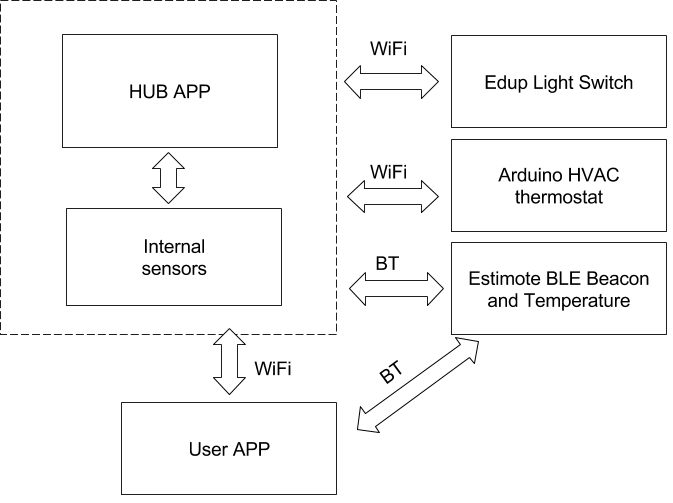
\includegraphics[width=0.7\textwidth]{Figures/top_view}
\caption{Architecture of the system}
\label{architecture_system}
\end{figure}





%This chapter is divided in three main sections. In Section 4.1 the detailed hardware architecture is
%described. Each of its subsection shows the decisions taken in the selection of the components.
%Section 4.2 describes the implementation of the software architecture. This section is composed of
%several subsections that detail the software configuration and explains the developed code.
%Finally, Section 3.5 details the deployment of the system in a set of offices at IST - Taguspark.

\subsection{Tablet}

A tablet capable of supporting a range of communication protocols and with some embedded sensors must be chosen as the base for the solution.

Several tablets were taken in consideration, the decisive factors were the price, \ac{CPU} speed/cores, \ac{RAM} and finally the supported communication protocols (\ac{BLE} and \ac{WiFi} are required). These factors are important since they allow the device to easier bought (price), allow multiple parallel complex computational operations like image processing, video recording, voice recognition (\ac{CPU} speed/cores and \ac{RAM}), devices with lower \ac{CPU} and \ac{RAM} may produce unexpected and unwanted results like crashes due to lack of resources. Since the device will be communication with a client device as talked about in section XXX (user app link......) it requires \ac{WiFi} to transfer and receive data and commands, \ac{BLE} can be used to receive external sensor data such as temperature.


Table~\ref{table:tablet} shows some examples of tablets running the major operating systems with similar hardware specifications.

In terms of price Apple tablets have the largest cost, since there is such a big gap in cost the iPad Mini 4 does not fit our needs. There are many types of Windows and Android tablets with very affordable prices. The Nexus was chosen because it was developed by Google in partnership with Asus, has very good reviews and is updated to the latest android version. There are Windows tablets cheaper than the HP ENVY 8 sold by Microsoft but there were a lack of reviews so a good tablet from a big manufacturer was picked.

The Android and Windows tablets have very similar hardware specifications. So the tablet chosen was the Nexus 7 (2013) since the programmer had previously developed Android apps.


\begin{table}[]
\centering
\begin{tabular}{|l|l|l|l|l|}
\hline
\textbf{name} & \begin{tabular}[c]{@{}l@{}}Apple iPad \\ mini 4\end{tabular} & Nexus 7 2013 & \begin{tabular}[c]{@{}l@{}}HP ENVY \\ 8 Note 5009\end{tabular} \\ \hline
\textbf{CPU speed} & 1.5 GHz & 1.5 GHz & 1.44 GHz \\ \hline
\textbf{CPU cores} & 2 & 4 & 4 \\ \hline
\textbf{RAM} & 2GB & 2GB & 2GB \\ \hline
\textbf{WiFi} & \begin{tabular}[c]{@{}l@{}}yes (2.4 GHz \\ and 5 GHz)\end{tabular} & \begin{tabular}[c]{@{}l@{}}yes (2.4 GHz \\ and 5 GHz)\end{tabular} & yes (2.4 GHz) \\ \hline
\textbf{BLE} & yes & yes & yes \\ \hline
\textbf{Light sensor} & yes & yes & yes \\ \hline
\textbf{Microfone} & yes & yes & yes \\ \hline
\textbf{Speaker} & yes & yes & yes \\ \hline
\textbf{Front camera} & yes & yes & yes \\ \hline
\textbf{Size} & \begin{tabular}[c]{@{}l@{}}7.9 inches (1536 \\ x 2048 pixels)\end{tabular} & \begin{tabular}[c]{@{}l@{}}7 inches (1200 \\ x 1920 pixels)\end{tabular} & \begin{tabular}[c]{@{}l@{}}8 inches (1200 \\ x 1920 pixels)\end{tabular} \\ \hline
\textbf{Operating System} & Apple IOS 10.0.1 & Android 6.0 & Windows 10 \\ \hline
\textbf{Cost (EUR)} & 449 & 131 & 178 \\ \hline
\end{tabular}
\caption{Comparison between some tablet devices}
\label{table:tablet}
\end{table}


\subsection{HVAC control}
In order for our \ac{BAS} solution to control an \ac{HVAC} system we would need to either communicate with a building central controlling unit or physically controlling the system like a thermostat does. Since many buildings don't have a central control point running some kind of server where you can control it using the internet, we went with the thermostat route.

For our smart thermostat to work we require a device capable of sending electric impulses to the \ac{HVAC} wire. 

Table~\ref{thermostat-choice} shows some commercial products and a Arduino solution.

We require a device that offers a  API in order to be controlled by our tablet, because the Sensi thermostat does not offer an official API it does not fit our requirements.

The Nest thermostat is the most popular option in the market integrated in many home automation systems, but since one of our requirements is keeping the cost low it does not fit our requirements. The path chosen was developing an Arduino solution with built in \ac{WiFi}, a relay to control the electric wires and a temperature and humidity sensor.



\begin{table}[]
\centering
\begin{tabular}{|l|l|l|l|}
\hline
\textbf{Name} & \begin{tabular}[c]{@{}l@{}}Sensi Wi-Fi \\ Thermostat\end{tabular} & \begin{tabular}[c]{@{}l@{}}Nest (3rd)\\ Thermostat\end{tabular} & \begin{tabular}[c]{@{}l@{}}Wemos D1 \\ mini Arduino + \\ Temperature Humidity \\ Sensor DHT11 + \\ Solid State Relay \\ 4 Channel + box\end{tabular} \\ \hline
\textbf{temperature/humidity} & yes & yes & yes \\ \hline
\textbf{Developer API} & no & yes & yes \\ \hline
\textbf{Cost (EUR)} & 116 & 223 & 4 + 1.5 + 6 + 1 = 12.5 \\ \hline
\end{tabular}
\caption{Differences between thermostat options.}
\label{thermostat-choice}
\end{table}


\subsection{Lighting control}
Besides controlling the room \ac{HVAC}, we require control over the lighting system. After some research we had three options: using wireless controllable light bulbs, using some kind of Arduino/relay solution like the thermostat or using a wireless controllable light switch.

Table~\ref{lighting-choice} show some available options.

Our lighting solution should be affordable, allow touch control and control using an API. The Philips Hue is costly and does not have lights supported by our office (fluorescent tube lamp) for these reasons it does not fit our requirements.

In order for our solution to be easily deplorable it requires the least amount of assembly and soldering components, an pre-built lighting product is preferable if the price range is close enough. Both the Arduino/relay and the DI-O/Arduino options have shortcomings, the first does not provide touch control and requires soldering and the latter also requires soldering in the Arduino interface side.

The lighting option chosen was the Edup Smart Light Switch, it provides touch control of the lighting, supports any existing infrastructure in existing buildings and is not too expensive.


Originally in Section \ref{architecture3} of the architecture, the lighting system was going to be integrated with the Arduino/\ac{HVAC} using relay actuators. We decided go with the Edup light switch after more searching for lighting products we could control, it is a better solution because of the touch control and no need for assembly as described previously.

\begin{table}[]
\centering
\begin{tabular}{|l|l|l|l|l|}
\hline
\textbf{Name} & \begin{tabular}[c]{@{}l@{}}Edup  - Wireless \\ Smart Home Wifi \\ Lighting Power\\ Switch\end{tabular} & \begin{tabular}[c]{@{}l@{}}Philips Hue Bridge + \\ light bulb +\\  light switch\end{tabular} & \begin{tabular}[c]{@{}l@{}}Wemos D1 \\ mini Arduino +  \\ Solid State Relay \\ 4 Channel + box\end{tabular} & \begin{tabular}[c]{@{}l@{}}DI-O - light \\ module + \\ DI-O double \\ light switch + \\ Wemos D1 \\ mini Arduino +\\  RF Transmitter \\ Receiver Module \\ 433MHz + box\end{tabular} \\ \hline
\textbf{manual control} & yes & yes & no & yes \\ \hline
\textbf{Developer API} & yes  (not officialy) & yes & yes & yes (arduino) \\ \hline
Wifi & yes & yes & yes & \begin{tabular}[c]{@{}l@{}}yes (needs arduino \\ to interface with \\ RF signals)\end{tabular} \\ \hline
\begin{tabular}[c]{@{}l@{}}Already built\\ (no extra work)\end{tabular} & yes & yes & no & \begin{tabular}[c]{@{}l@{}}no (needs arduino \\ and RF components \\ to be built)\end{tabular} \\ \hline
\begin{tabular}[c]{@{}l@{}}Support for \\ any office \\ (any light bulb)\end{tabular} & yes & no & yes & yes \\ \hline
\textbf{Cost (EUR)} & 27.93 & 56,31 +39,34 = 95,65 & 4 + 6 + 1 = 11 & \begin{tabular}[c]{@{}l@{}}18,40 + 24,40 + 4 \\ + 0,5 +1 = 48,3\end{tabular} \\ \hline
\end{tabular}
\caption{Lighting control options.}
\label{lighting-choice}
\end{table}


\subsection{Bluetooth Beacon}

We require a way to determine if a user is near a certain point in the building such as the office. In section XXX this will be approach in higher detail.

From the alternatives seen in Section~\ref{ocupacy_detection}, we  determined that \ac{BLE} beacons an option to achieve room base location in a building.

There are many kinds of devices capable of emitting \ac{BLE} packets: android devices( available in version 5.0), some microcontrolers and commercial beacon products.

We decided to use a Estimote beacon, the reason it was chosen was because we had one extra around. Since it is portable we can position it anywhere in the room, enabling better coverage, as it does not need to be connected to a power socket.








\section{Software Architecture}

\subsection{HUB APP}

\begin{figure}[h]
\centering
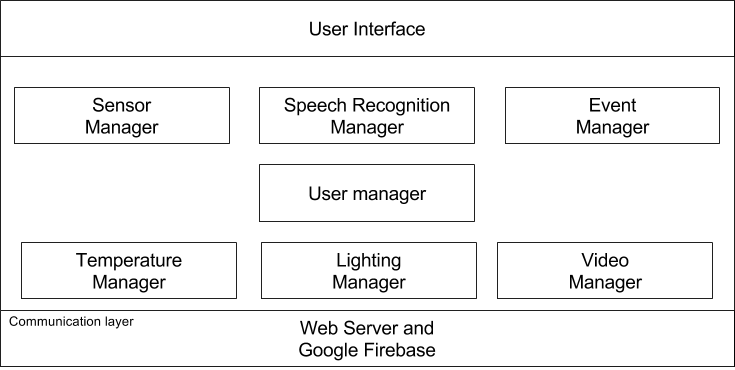
\includegraphics[width=0.7\textwidth]{Figures/software_implementation}
\caption{Software architecture of HUB APP}
\label{software_imp}
\end{figure}

There were a couple of changes in regard to the starting software architecture, we will present the current implementation:

\paragraph{Event Manager}\mbox{}\\

The Event Manager  operates in a publish/subscriber basis. Other managers register their interest in certain events and when whose events happen they are notified. The events can be published to the event manager by any other manager. For example the Sensor Manager can publish and motion detected event, that the video manager is interested.

Currently there are eight different events available:

\begin{itemize}
  \item \textbf{Temperature:} Contain the current temperature and humidity.
  \item \textbf{Motion:} This event contains a boolean to inform if movement is detected, and long value with the time since last movement was detected.
  \item \textbf{Speech:} The phrase of an successful speech recognition.  
  \item \textbf{Time:} If we need to check some task regularly this event is triggered every 2 seconds.  
  \item \textbf{User location:} This event contains the user id, the location type (Office/Building), a boolean to specify if he is in the location or left and finnaly a boolean.
  \item \textbf{Brightness:} The value in Lux of the light sensor.  
  \item \textbf{Light:} The light number and it's status. 
  \item \textbf{Change temperature:} The value of temperature we want the thermostat to be at. 
  
\end{itemize}


The Event Manager also receives a list a recipes created by the user. These recipes contain a list a trigger and actions. When a event is published all the recipes are examined to see if all triggers conditions are fulfilled. When this happens all the actions in that particular recipe are executed.

There are six triggers available:

\begin{itemize}
  \item \textbf{Temperature:} This trigger allows the user to trigger an action when the office temperature is bellow or above a value specified.
  \item \textbf{Motion:} The motion sensor is triggered when something changes in the field of view of the assistant or no movement detected in X seconds.
  \item \textbf{Speech:} Say the keyword "my assistant" and after the beep you say the phrase specified in the trigger.  
  \item \textbf{Time:} The timer trigger allows the user to run certain actions at a specific time(Scheduler).  
  \item \textbf{User location:} Allows the user to choose from a list of different scenarios ("User is inside office", "User is inside building", "User leaves office", "User leaves building", "User arrives at office", "No user inside building", "No user inside office" and "User arrives at building").
  \item \textbf{Light sensor:} The light sensor triggers an action if the light level is bellow or above the value specified.
  
\end{itemize}

The actions available are:

\begin{itemize}
  \item \textbf{Light:} Sets the state of the lights.
  \item \textbf{Temperature:} Changes the target temperature and turns on the HVAC if needed.
  \item \textbf{Speech:} This action uses the speakers to say the text specified (text to speech).
\end{itemize}


\paragraph{Speech Recognition Manager}\mbox{}\\

This manager uses the CMU Sphinx offline keyword speech recognizer, meaning it will detect one word in our case "my assistant". When it detects the keyword it shuts down and we launch google online speech recognition. We use this other speech recognition because it offer good results, the reason the manager uses two different speech recognizes is because using only google recognizer has higher bandwidth cost since we would be constantly sending audio.The other reason is privacy, we don't know if google is going to disclose our audio files to third parties.

When we successfully say the keyword a beep sound is played and google speech recognizer listens to the rest of the voice command, when the results arrive from google they are published to the Event manager.

There were several problems with both recognizer, the Sphinx has a lot of false positives for small words, for our current keyword we sometimes need to repeat more than once for it to recognize. This problem can perhaps be attributed to the fact we are not native English speakers. 
Google speech recognizer is plagued with problems since a few version ago, it sometimes will not listen and shutdown after some 100 ms. To try to minimize the problem by run a check every 10 seconds. If both speech recognizes are not running we relaunch Sphinx.

\paragraph{Sensor Manager}\mbox{}\\

The Sensor Manager is responsible for the light sensor and virtual motion sensor.

The light sensor is built in in the tablet. Every 2 seconds the current light level is published to the Event manager. 

Since the tablet does not have a motion sensor, we use the front camera and analyze the frames every second. If the total number of the RGB pixels with threshold above 50 is different we know there was a change in the eye sight of the camera. The percentage of different pixels for a positive detection is user defined, the default is 0.5%.

A problem that motion detecting cameras have are the false positives specially when there is a windows to the outside. A strong light can trigger the sensor, because of that we designed the sensor be able to ignore an area of the camera frame. It is possible to specify the area to ignore in the HUB APP settings.


\paragraph{Video Manager}\mbox{}\\

The Video manager does two jobs, it records 30 seconds videos when no user is present in the office and motion is detected. The other job is offering a live preview of the office, an user can use the USER APP to watch in real time the office.

The recorded videos don't have any audio because Android does not allow the audio to be shared between the speech recognizer and the video recorder at the same time.

The video manager can be enabled and disabled in the HUB settings for privacy reasons.



\paragraph{Lighting Manager}\mbox{}\\

\paragraph{Temperature Manager}\mbox{}\\

\paragraph{User Manager}\mbox{}\\


\paragraph{Web Server and Google Firebase}\mbox{}\\


\subsection{USER APP}







